\documentclass[book]{standalone}

\usepackage{import} % Required for importing other .tex docs.  (import uses everything bw Begin and End Doc)
\usepackage{float} % Required for specifying the exact location of a figure or table
\usepackage{graphicx} % Required for including images
\usepackage{wrapfig}
\usepackage[pdftex,breaklinks,colorlinks=true,linkcolor=black,citecolor=blue,urlcolor=red,linktocpage=false,pagebackref=true,filecolor=magenta]{hyperref}%http://www.tug.org/applications/hyperref/manual.html#x1-100003.6
\usepackage{cite}
\usepackage[toc,title,page]{appendix}
\usepackage{pdfpages} % enables loading a pdf into the doc
\usepackage{makeidx}
\usepackage{glossaries} % must be after hyperref
\usepackage{blindtext}
\usepackage{enumitem}
%\usepackage{caption}

%\setlist[description]{leftmargin=\parindent,labelindent=\parindent}

%\renewcommand*{\bibname}{References} % renames the bibliography

\newcommand{\HRule}{\rule{\linewidth}{0.5mm}} % Command to make the lines in the title page

\graphicspath{{img/}{GIS_ChampionSection/img/}{awardsChapter/GIS_ChampionSection/img/}{brandPart/awardsChapter/GIS_ChampionSection/img/}{img/}{pairedProgSection/img/}{methodChapter/pairedProgSection/img/}{methodPart/methodChapter/pairedProgSection/img/}{documentationSection/img/}{methodChapter/documentationSection/img/}{methodPart/methodChapter/documentationSection/img/}{docStorageOrgSection/img/}{methodChapter/docStorageOrgSection/img/}{methodPart/methodChapter/docStorageOrgSection/img/}{QGisSection/img/}{toolsChapter/QGisSection/img/}{servicePart/toolsChapter/QGisSection/img/}{ESRISection/img/}{toolChapter/ESRISection/img/}{servicePart/toolChapter/ESRISection/img/}{../../../../source/}{../../source/}{servicePart/applicationsChapter/treasurerSection/img/}}

%\setlength\parindent{0pt} % eliminates indents


\def\titlename{Using Northing And Easting From Plans}

\title{\HRule % Horizontal Line added
\\[.4cm] % space
\begin{figure}[H] % included image
\begin{center}	% centered horizontally
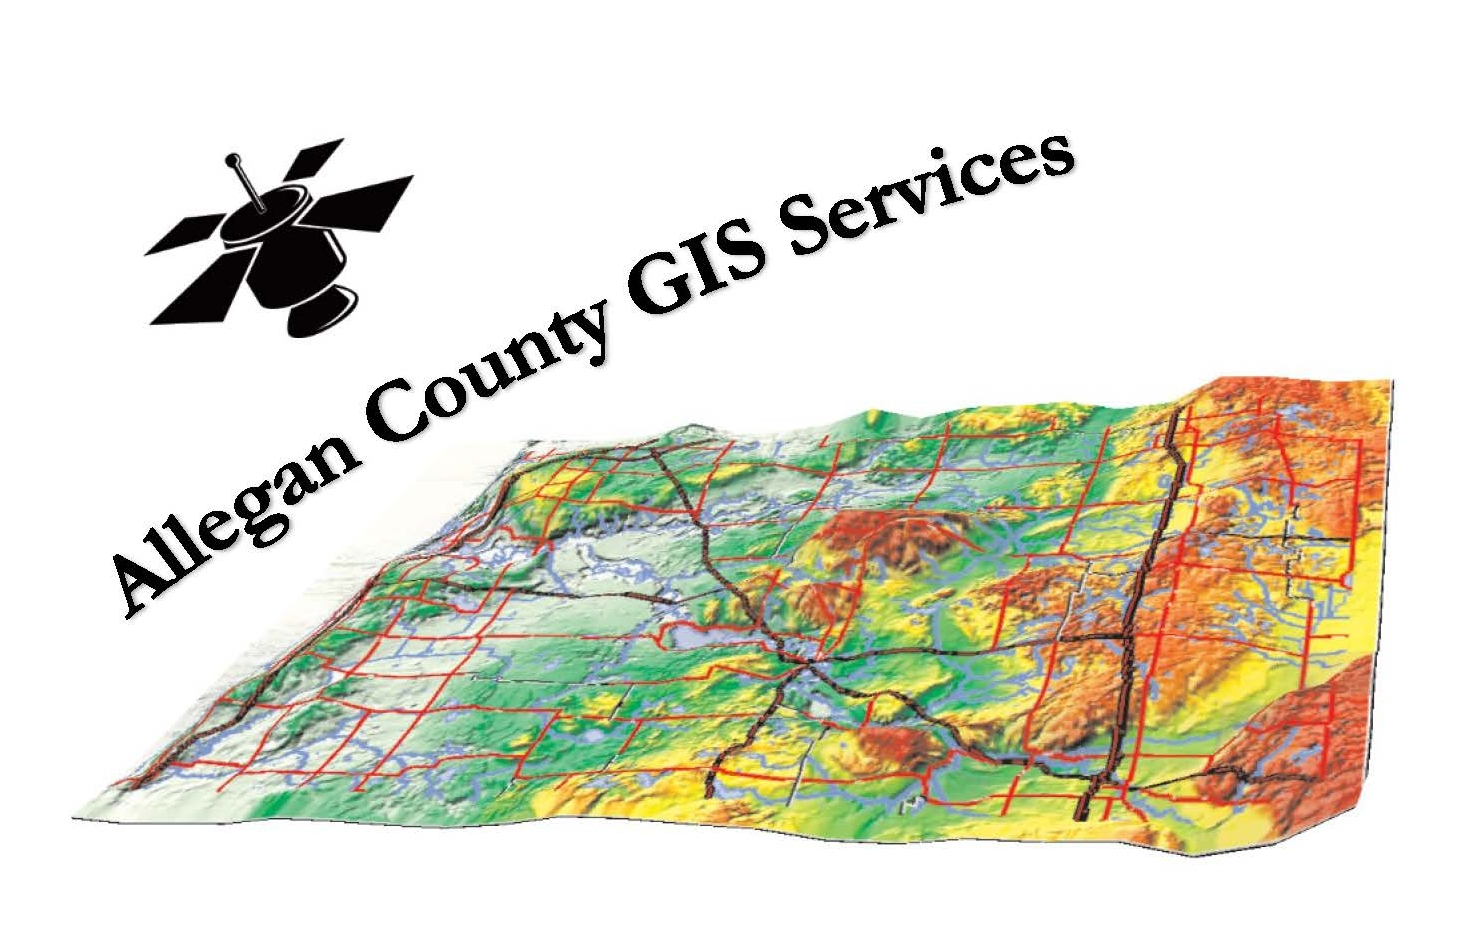
\includegraphics[scale=.45]{GIS_Logo_better.jpg}
\end{center}
\end{figure}
\Huge \bfseries \titlename \\ % Title text
\HRule \\[.4cm] % Horizontal Line added
\author{\Large Allegan County GIS \\\Large www.allegancounty.org/gis} % defines author
}  % inputs common title
\setcounter{tocdepth}{5}  % subparagraph and down
\begin{document}% document begins

\ifstandalone
%\frontmatter % turns off chapter numbering and uses roman numerals for page numbers
\maketitle % creates title page and blank page after title page
\tableofcontents % creates TOC and blank page
\clearpage
%\mainmatter % turns on chapter numbering, resets page numbering and uses arabic numerals for page numbers
\fi
\clearpage
\subsection{Northing And Easting}
\medskip
\subsubsection[How to use]{How to use Northing and Easting}
\vspace{.1in}

\paragraph[Use a Spreadsheet]{}\textbf{{\Large Using a spreadsheet to convert the dimensions}}
\vspace{.1in}

%{\Large $\Rightarrow$ Push the Configure Button}
%
%
\noindent To use Northing and Easting from survey plans:\\
\vspace{.1in}

\noindent In a spreadsheet, adjust the data to be relative to the 1st point\\
\vspace{.1in}

\noindent So if a survey gives you:\\

\begin{table}[htbp]
\centering
\resizebox{.5\linewidth}{!}{%
\begin{tabular}{|c|c|c|}
\hline
Pt&Northing&Easting\\ \hline
1&995.9952&9766.6\\
2&994.3049&9112\\
3&989.234&7150\\
4&1194.3099&9114\\
5&1193.266&8710.2059\\
6&1193.0954&8644.2016\\
...&...&...\\
32&1617.7856&8827.4296\\
\hline
\end{tabular}
}
\caption{Survey Plan Northing and Easting}
\end{table}
\clearpage

\noindent Calculate Relative North and Relative Easting of the points to Point 1 by subtracting the point 1 values from each of the other points.\\
\vspace{.1in}

\noindent Use formulas:

\begin{table}[htbp]
\centering
\resizebox{.75\linewidth}{!}{%
\begin{tabular}{|c|c|c|c|c|c|}
\hline

 &A&B&C&D&E\\\hline
1&Pt&Northing&Easting&Relative NS&Relative EW\\
2&1&995.9952&9766.6&0&0\\
3&2&994.3049&9112&=B3-B\textdollar2&=C3-C\textdollar2\\
4&3&989.234&7150&=B4-B\textdollar2&=C4-C\textdollar2\\
...&...&...&...&...&...\\
6&32&1617.7856&8827.4296&=B9-B\textdollar2&=C9-C\textdollar2\\
\hline
\end{tabular}
}
\caption{Survey Plan Northing and Easting}
\end{table}

Giving you:

\begin{table}[htbp]
\centering
\resizebox{.75\linewidth}{!}{%
\begin{tabular}{|c|c|c|c|c|c|}
\hline
 &A&B&C&D&E\\\hline
1&Pt&Northing&Easting&Relative NS&Relative EW\\
2&1&995.9952&9766.6&0&0\\
3&2&994.3049&9112&-1.6903&-654.6\\
4&3&989.234&7150&-6.7612&-2616.6\\
...&...&...&...&...&...\\
6&32&1617.7856&8827.4296&621.7904&-939.1704\\
\hline
\end{tabular}
}
\caption{Relative Northing and Easting}
\end{table}

So to place pt 32:\\

From pt 1:\\

Use distances 621.7904' N and 939.1704'W

\end{document}
